%%%
% set up document type
%%%
\documentclass[12pt]{article}

%%%
% declare all packages
%%%
\usepackage[left=25mm, top=20mm, right=25mm, bottom=30mm,nohead,nofoot]{geometry} 

\usepackage[T2A]{fontenc}
\usepackage[utf8]{inputenc}
\usepackage[english, russian]{babel}

\usepackage{graphics, graphicx}

\usepackage{url}
\usepackage{hyperref}

\usepackage{amssymb,latexsym} 
\usepackage{MnSymbol}
\usepackage{mathrsfs}

\usepackage[nottoc,numbib]{tocbibind}
\usepackage{float}
\usepackage{listings}
\usepackage{multirow}
\usepackage{hhline}

\usepackage{color,colortbl}

% \usepackage{verbatim}
%%%
% document settings
%%%
\setcounter{tocdepth}{4}
\graphicspath{ {./pic/} }

\renewcommand{\listoffigures}{\begingroup  % add number to list of graphics
\tocsection
\tocfile{\listfigurename}{lof}
\endgroup}
\renewcommand{\listoftables}{\begingroup  % add number to list of tables
\tocsection
\tocfile{\listtablename}{lot}
\endgroup}

%******************************************************************
%******************************************************************
\begin{document}

\begin{titlepage}
	\center
		Санкт-Петербургский Политехнический 
		университет \\ Петра Великого\\
		Институт прикладной математики и механики
		\\ \textbf{Кафедра «Прикладная математика»}

	\vfill ~
	\textbf{
		\\ \large ЛАБОРАТОРНАЯ РАБОТА №1
	}
	\\	на тему 
	\\ "Метод конечных разностей для ОДУ 2-го порядка"
	\\ по дисциплине
	\\ "Конечно-разностные и сеточные методы"

	\vfill ~

	Выполнил студент гр. \textbf{3630102/60101} \\
	\textbf{Лансков.Н.В.} \\ 

\vfill

{\large}	Санкт-Петербург
\\ 2019
\end{titlepage}

%%%
% Table of conetnts 
%%%

\tableofcontents 
\newpage
\listoffigures
\newpage
\listoftables
\newpage

%%%
% Text
%%%
\section{Постановка задачи}

Рассмотрим задачу :

$$
\begin{cases}
-\dfrac{d^2u}{dx^2} + e^x\dfrac{du}{dx} + u(cos^2(x) + 1) = f(x), & x \in [0;2] \\ \\
\dfrac{du}{dx}(0.5) + u(0.5) = e^{0.5}sin(e^{0.5}) - cos(e^{0.5}) \\ \\
\dfrac{du}{dx}(2) + u(2) = e^2cos(e^2) + sin(e^2)
\end{cases}
$$

Где:
$$
f(x) = -e^xcos(e^x) + e^{2x}sin(e^x) + e^{2x}cos(e^x) + sin(e^x)(sin^2(x) + 1)
$$

Точное решение задачи - $u(x) = sin(e^x)$ 
\section{Разностные схемы}
\subsection{Разностная схема $O(h^2)$}
Введём регулярную сетку:
$$
\Omega_h(x) = \{x_i | x_i = ih, i = \overline{0, M}, h = \dfrac{1}{M}\}
$$

Выбор шага h будет осуществляться несколько раз для сравнения полученных результатов при различных шагах.
Выберем следующий шаблон аппроксимации:
$$
\omega_h(x_i) = \{ x_{i-1}; x_i; x_{i + 1}\}
$$

при выборе данного шаблона для аппроксимации первой и второй производной  мы получим требуемую погрешность . Для такого шаблона ранее были выведены аппроксимации первой и второй производных, а именно:

$$
u_{\dot{x}} = \dfrac{u_{i + 1} - u_{i - 1}}{2h}
$$

$$
u_{\overline{x}x} = \dfrac{u_{i + 1} -2u_i+ u_{i - 1}}{h^2}
$$

Тогда можем переписать исходную задачу, используя сеточную функцию v(x) – приближение к u(x) следующим образом:

$$
\begin{cases}
-\dfrac{v_{i+1} - 2v_i + v_{i-1}}{h^2} + e^x\dfrac{v_{i+1} - v_{i-1}}{2h} + v_i(sin^2(x) + 1) = f_i^* \\
\\
- \dfrac{-3v_0 + 4v_1 - v_2}{2h} + v_0 = sin(1) - cos(1) \\
\\
\dfrac{3v_M - 4v_{M-1} + v_{M-2}}{2h} + v_M = e^2cos(e^2) + sin(e^2)
\end{cases}
$$

Стоит обратить внимание на аппроксимацию на краях отрезка, для них используется другие шаблоны аппроксимации:
$$
\omega_h(x_i) = \{ x_{i}; x_{i + 1}; x_{i + 2}\}
$$

$$
\omega_h(x_i) = \{ x_i; x_{i - 1}; x_{i - 2}\}
$$

Ранее доказано, что выбор данных шаблонов аппроксимации обеспечит нам общую погрешность разностной схемы как 
$O(h^2)$

Тогда, перегруппировав слагаемые, получим СЛАУ, которую будем решать методом прогонки, у искомой СЛАУ получим трехдиагональную матрицу коэффициентов.

$$
\begin{cases}
v_{i-1}(-\dfrac{1}{h^2} - \dfrac{e^{x_i}}{2h}) + v_i(\dfrac{2}{h^2} + sin^2(x_i) + 1) + v_{i + 1}(-\dfrac{1}{h^2} + \dfrac{e^{x_i}}{2h}) = f_i^*\\
\\
v_o(\dfrac{3}{2h}  +1) + v_1(-\dfrac{2}{h}) + v_2(\dfrac{1}{2h}) = e^{0.5}sin(e^{0.5}) - cos(e^{0.5})\\
\\
v_{M-2}(\dfrac{1}{2h}) + v_{M-1}(-\dfrac{2}{h})  +v_M(\dfrac{3}{2h} + 1) = e^2cos(e^2) + sin(e^2)
\end{cases}
$$

В итоге получена матрица коэффициентов:

$$
\begin{pmatrix}
	\dfrac{3}{2h}  +1 & -\dfrac{2}{h} &  \dfrac{1}{2h} & 0 & ... \\
	\\
	-\dfrac{1}{h^2} - \dfrac{e^{x_2}}{2h} & \dfrac{2}{h^2} + sin^2(x_2) + 1 & -\dfrac{1}{h^2} + \dfrac{e^{x_2}}{2h} & 0 & ... \\
	\\
	0 & -\dfrac{1}{h^2} - \dfrac{e^{x_3}}{2h} & \dfrac{2}{h^2} + sin^2(x_3) + 1 & -\dfrac{1}{h^2} + \dfrac{e^{x_3}}{2h} & ... \\
	... & ... & ... & ... & ... \\
	\\
	... & 0 & -\dfrac{1}{h^2} - \dfrac{e^{x_{M-1}}}{2h} & \dfrac{2}{h^2} + sin^2(x_{M-1}) + 1 & -\dfrac{1}{h^2} + \dfrac{e^{x_{M-1}}}{2h} \\
	\\
	... & 0 & \dfrac{1}{2h} & -\dfrac{2}{h} &\dfrac{3}{2h} + 1 \\
\end{pmatrix}
$$

С правой частью из $sin(1) - cos(1), e^2cos(e^2) + sin(e^2)$ и  $f_i^*$ для $i = \overline{2, M-1}$. Для того, чтобы решить данную СЛАУ методом прогонки и получить искомый результат, необходимо привести матрицу к трехдиагональному виду. Домножаем вторую строку на выражение $ - \dfrac{\dfrac{1}{2h}}{-\dfrac{1}{h^2} + \dfrac{e^{x_2}}{2h}} $ (с учётом правой части!) и прибавляем к первой. Аналогичным образом поступаем для "правки" последней строки. В результате получается трёхдиагональная матрица, которая уже непосредственно используется в методе прогонки:


$$
\begin{pmatrix}
	(\dfrac{3}{2h}  +1)( - \dfrac{\dfrac{1}{2h}}{-\dfrac{1}{h^2} + \dfrac{e^{x_2}}{2h}})& 
	(-\dfrac{2}{h})( - \dfrac{\dfrac{1}{2h}}{-\dfrac{1}{h^2} + \dfrac{e^{x_2}}{2h}}) &  0 & 0 & ... \\
	\\
	-\dfrac{1}{h^2} - \dfrac{e^{x_2}}{2h} & \dfrac{2}{h^2} + sin^2(x_2) + 1 & ... & 0 & ... \\
	\\
	0 & -\dfrac{1}{h^2} - \dfrac{e^{x_3}}{2h} & ... & -\dfrac{1}{h^2} + \dfrac{e^{x_3}}{2h} & ... \\
	... & ... & ... & ... & ... \\
	\\
	... & 0 & ... & \dfrac{2}{h^2} + sin^2(x_{M-1}) + 1 & -\dfrac{1}{h^2} + \dfrac{e^{x_{M-1}}}{2h} \\
	\\
	... & 0 & 0 & (-\dfrac{2}{h})( - \dfrac{\dfrac{1}{2h}}{-\dfrac{1}{h^2} - \dfrac{e^{x_{M-1}}}{2h}}) &
	(\dfrac{3}{2h} + 1)( - \dfrac{\dfrac{1}{2h}}{-\dfrac{1}{h^2} - \dfrac{e^{x_{M-1}}}{2h}}) \\
\end{pmatrix}
$$

\subsection{Разностная схема $O(h)$}

Аналогично предыдущему пункту, выберем сетку:
Для этого введем регулярную сетку:

$$
\Omega_h(x) = \{x_i | x_i = ih, i = \overline{0, M}, h = \dfrac{1}{M}\}
$$

причем выбор шага h будет осуществляться несколько раз для сравнения полученных результатов при различных шагах.
Для второй производной выберем использованный ранее шаблон аппроксимации, для первой производной шаблон апроксимации будет иметь вид:
$$
\omega_h(x_i) = \{ x_{i}; x_{i + 1}\}
$$
Тогда :
$$
u_x = \dfrac{u_{i + 1} + u_{i}}{h^2}
$$

Проводя аналогичные предыдущему пункту рассуждения, перейдем от исходной задачи к разностной схеме. В этом случае, так как нам требуется точность всего лишь O(h), то условия на границах можно аппроксимировать чуть более простой разностной схемой с тем же шаблоном, что используется для аппроксимации первой производной.

$$
\begin{cases}
- \dfrac{v_{i+1} - 2v_i + v_{i - 1}}{h^2} + e^{x_i}\dfrac{v_{i+1} - v_i}{h} + v_i(sin^2(x) + 1) = f_i^* \\
\\
- \dfrac{v_1 - v_0}{h} + v_0 = sin(1) - cos(1) \\
\\
\dfrac{v_M - v_{M-1}}{h} + v_M = e^2cos(e^2) + sin(e^2)
\end{cases}
$$


Иными словами, сразу получаем трёхдиагональную матрицу. Решаем методом прогонки.

$$
\begin{pmatrix}
	\dfrac{1}{h} + 1& -\dfrac{1}{h} &  0 & 0 & ... \\
	\\
	-\dfrac{1}{h^2}  & \dfrac{2}{h^2} - \dfrac{e^{x_2}}{h} + sin^2(x_2) + 1 & -\dfrac{1}{h^2} + \dfrac{e^{x_2}}{h} & 0 & ... \\
	\\
	0 & -\dfrac{1}{h^2} & \dfrac{2}{h^2} - \dfrac{e^{x_3}}{h} + sin^2(x_3) + 1 &
	 -\dfrac{1}{h^2} + \dfrac{e^{x_3}}{h} & ... \\
	... & ... & ... & ... & ... \\
	\\
	... & 0 & \dfrac{-1}{h^2} & \dfrac{2}{h^2} - \dfrac{e^{x_3}}{h} + sin^2(x_3) + 1 &
	 -\dfrac{1}{h^2} + \dfrac{e^{x_{M-1}}}{h} \\
	\\
	... & 0 & 0 & -\dfrac{1}{h} & \dfrac{1}{h} + 1\\
\end{pmatrix}
$$

\section{Результаты}

\subsection{Разностная схема $O(h^2)$}

Для определения погрешности найдем следующую норму:
$$
||z_h|| = || u_h - v_h ||
$$
Норму будем вычислять по формуле:
$$
||x|| = \sqrt{h\sum\limits_{i=1}^M x_i^2}
$$

\begin{figure}
\begin{center}
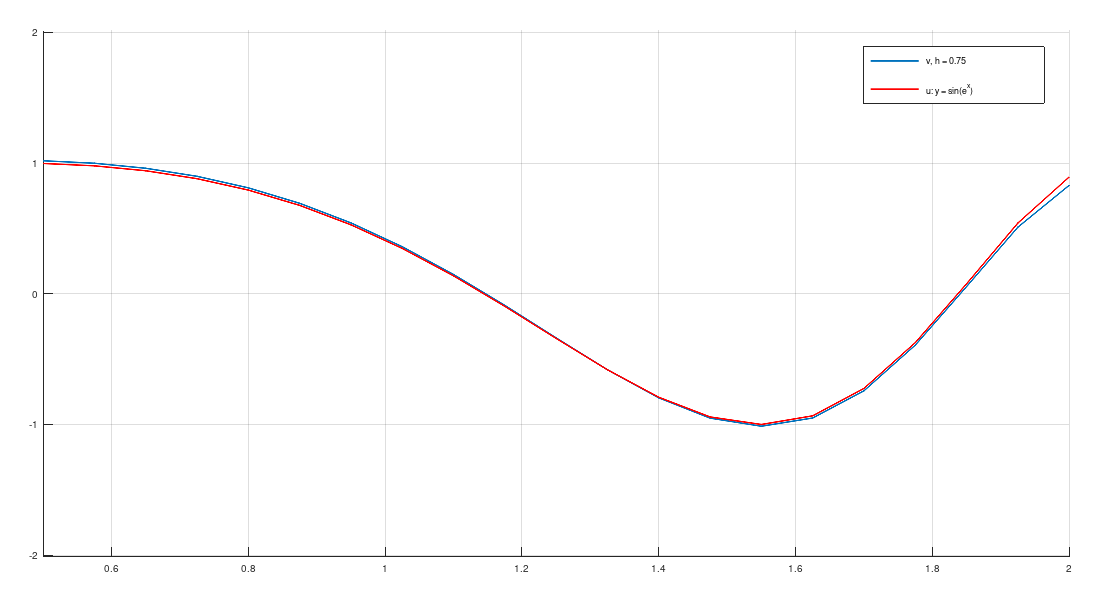
\includegraphics[scale = 0.4]{h2_20.png} 
\end{center}
\caption{$O(h^2), n = 20$ }
\end{figure}

\begin{figure}
\begin{center}
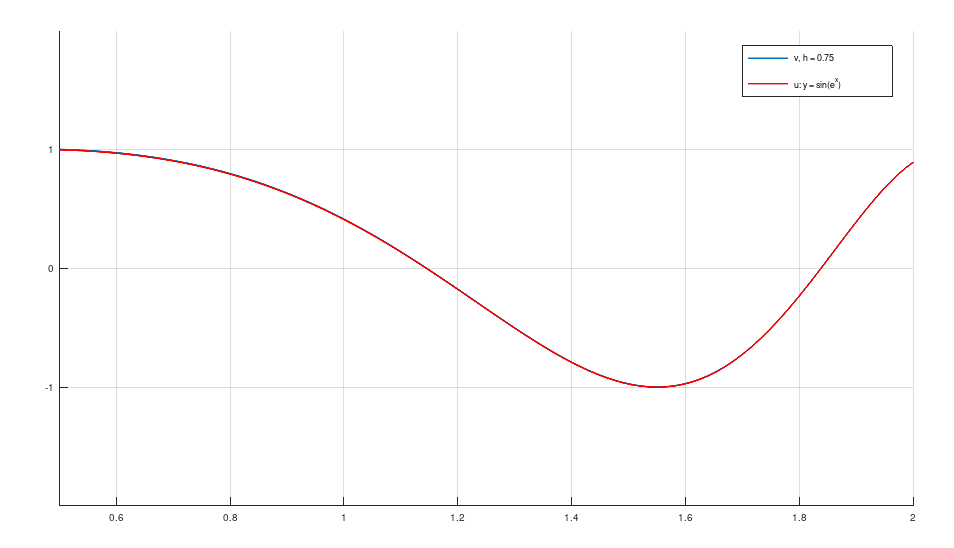
\includegraphics[scale = 0.4]{h2_100.png} 
\end{center}
\caption{$O(h^2), n = 100$ }
\end{figure}

\begin{table}[H]
\caption{Зависимость погрешности от числа узлов}
\begin{center}
\begin{tabular}{|c|c|c|}
\hline
\textit{Число узлов} &$ h$ & $||z_h||$  \\
\hline
20 & 0.75 & 0.0200350 \\
\hline
40 & 0.0375 & 0.0071457 \\
\hline
100 & 0.015 & 0.0041768 \\
\hline
1000 & 0.0015 & 0.0028642 \\
\hline
10000 & 0.00015 & 0.0027157 \\
\hline
65536 & 0.000022888 & 0.0027014 \\
\hline
1000000 & 0.0000015000 & 0.0026990 \\
\hline
\end{tabular}
\end{center}
\end{table}

\subsection{Разностная схема $O(h)$}

\newpage
\begin{figure}
\begin{center}
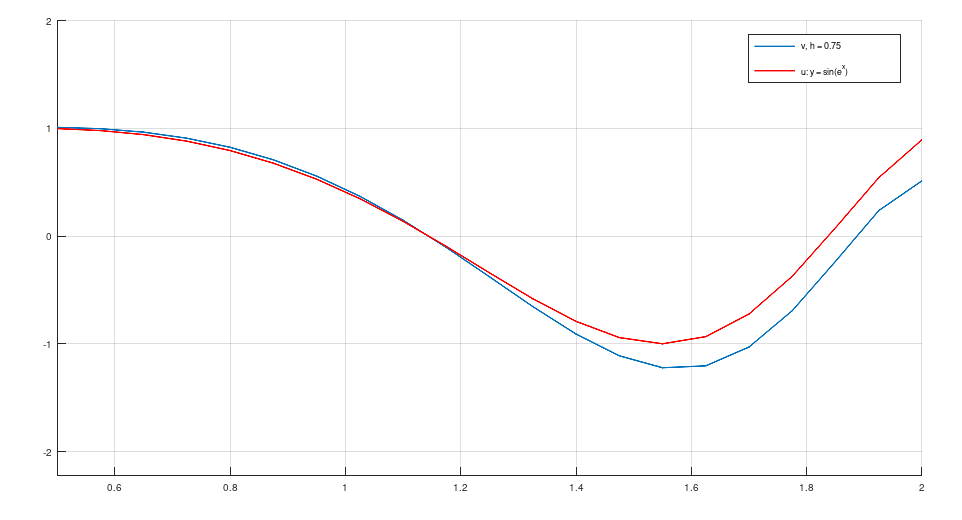
\includegraphics[scale = 0.4]{h_20.png} 
\end{center}
\caption{$O(h), n = 20$ }
\end{figure}

\newpage
\begin{figure}
\begin{center}
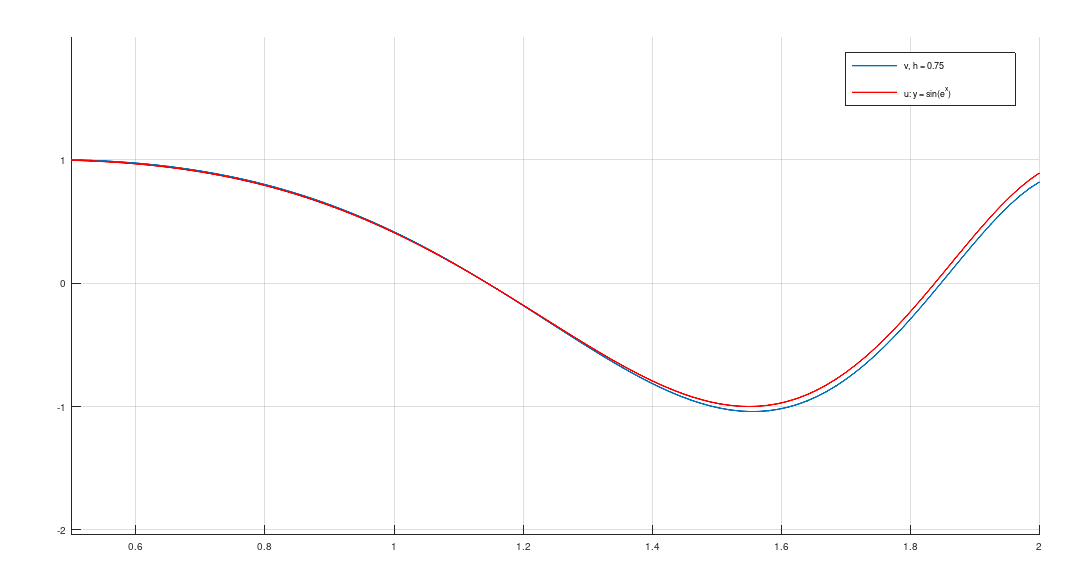
\includegraphics[scale = 0.4]{h_100.png} 
\end{center}
\caption{$O(h), n = 100$}
\end{figure}

\newpage
\begin{table}[H]
\caption{Зависимость погрешности от числа узлов}
\begin{center}
\begin{tabular}{|c|c|c|}
\hline
\textit{Число узлов} &$ h$ & $||z_h||$  \\
\hline
20 & 0.75 & 0.2055764 \\
\hline
40 & 0.0375 & 0.1030405 \\
\hline
100 & 0.015 & 0.0407417 \\
\hline
1000 & 0.0015 & 0.0037649\\
\hline
10000 & 0.00015 & 0.0025252 \\
\hline
65536 & 0.000022888 & 0.0026688 \\
\hline
\end{tabular}
\end{center}
\end{table}

\subsection{Зависимости погрешности от шага}

% \begin{table}[H]
% \caption{Зависимость погрешности от числа узлов}
% \begin{center}
% \begin{tabular}{|c|c|c|}
%\hline
%\textit{Число узлов} &$ h$ & $||z_h||$  \\
%\hline
%20 & 0.75 & 0.0200350 \\
%\hline
%40 & 0.0375 & 0.0071457 \\
%\hline
%\end{tabular}
%\end{center}
%\end{table}

\section{Выводы}


\end{document}

